\documentclass[11pt]{article}
\usepackage{apchem}
\doctitle{Unit 3 Content Guide}
\docsubtitle{A Comprehensive Review of Properties of Substances and Mixtures, Topics 3.1--3.13}
\docstatus{Study draft}
\begin{document}
\titleblock
\begin{abstract}
This guide covers all of Unit 3, Properties of Substances and Mixtures, in fourteen sections: one for each of Topics 3.1--3.13 in course order, plus a final section on lab skills and free-response technique. Each section gives the definitions, equations and particle-level reasoning the topic needs, at least one worked example, the phrasing that earns free-response points and the mistakes that cost them. The worked examples use their own numbers, so none of them give away an item in \emph{Unit 3 Practice Set A} or \emph{Unit 3 Practice Set B}; the answer keys of both sets point back to the section numbers here. Unit 3 is the heaviest unit on the exam, so plan on about 90 minutes for a full read with a calculator out.
\end{abstract}
\leadline{Usage}{first pass, read Sections 1--14 in order and redo every worked example. Then take \emph{Unit 3 Practice Set A} cold; reread the section behind every miss, and take \emph{Unit 3 Practice Set B} two or three days later. The last page is a one-page summary for the night before the unit test. Unit 3 is 18--22\% of the AP multiple-choice section, the largest share of any unit.}

\section{Intermolecular and interparticle forces (Topic 3.1)}\label{t:3.1}
Intermolecular forces (IMFs) are attractions \emph{between} particles. They are much weaker than covalent or ionic bonds, and they decide boiling points, vapor pressures, solubility and viscosity.
\begin{center}
\begin{tabular}{p{0.22\linewidth}p{0.38\linewidth}p{0.30\linewidth}}\toprule
Force & Between & Strength depends on \\ \midrule
London dispersion & all molecules (temporary, induced dipoles) & number of electrons (polarizability), contact area \\
Dipole--dipole & polar molecules (permanent dipoles) & size of the dipole \\
Hydrogen bonding & H bonded to N, O or F, and a lone pair on N, O or F & number of H-bonds per molecule \\
Ion--dipole & an ion and a polar molecule & ion charge, closeness \\ \bottomrule
\end{tabular}
\end{center}
\begin{itemize}
\item Every molecule has dispersion forces. For large molecules they can outweigh dipole--dipole forces in small ones (CCl$_4$, nonpolar, boils at 77 \textdegree C; HCl, polar, at $-85$ \textdegree C).
\item Hydrogen bonds are especially strong dipole--dipole attractions. The H must be covalently bonded to N, O or F; an H on carbon does not hydrogen-bond.
\item To compare substances, first compare size (electrons). If sizes are similar, the type of strongest IMF decides. If both are similar, shape (contact area) decides.
\end{itemize}
\worked{1.1} Rank by boiling point: $\ce{CH3CH2CH2CH3}$ (butane), $\ce{CH3CH2CH2OH}$ (1-propanol), $\ce{CH3COCH3}$ (acetone). All have about 32--34 electrons. Butane: dispersion only (lowest, $-1$ \textdegree C). Acetone: dipole--dipole (56 \textdegree C). 1-propanol: hydrogen bonding (97 \textdegree C).

\frph Name the specific IMF in each substance, say which is stronger and why (``more electrons, more polarizable'' or ``O--H allows hydrogen bonding''), and connect it to the property: ``more energy is needed to separate the molecules.'' Never say ``bonds break'' when a molecular substance boils.

\errorsh
\begin{itemize}
\item Saying a C--H bond can hydrogen-bond.
\item Saying nonpolar molecules have ``no'' IMFs. They have dispersion forces.
\item Explaining boiling with the strength of covalent bonds inside the molecule.
\end{itemize}

\section{Properties of solids (Topic 3.2)}\label{t:3.2}
\begin{center}
\begin{tabular}{p{0.15\linewidth}p{0.2\linewidth}p{0.17\linewidth}p{0.18\linewidth}p{0.18\linewidth}}\toprule
Solid & Particles and forces & Melting point & Conductivity & Example \\ \midrule
Ionic & ions; ionic bonds & high & melted or dissolved only & KCl \\
Metallic & cations, e$^-$ sea & varies & yes & Al \\
Network covalent & atoms; covalent bonds & very high & no (graphite: yes) & diamond, SiC, $\ce{SiO2}$ \\
Molecular & molecules; IMFs & low & no & ice, $\ce{CO2}$, sucrose \\ \bottomrule
\end{tabular}
\end{center}
Crystalline solids have a repeating pattern and a sharp melting point; amorphous solids (glass, many plastics) have no long-range order and soften over a range of temperatures.

Graphite is a network solid with layers of $sp^2$ carbon atoms. Delocalized $\pi$ electrons in each layer conduct electricity, and only dispersion forces hold the layers together, so they slide (a lubricant, pencil ``lead'').

\worked{2.1} A white solid melts at 133 \textdegree C, dissolves in water, and its solution does not conduct. It is a polar molecular solid (for example, urea), not an ionic solid, because ionic solutions conduct and ionic solids melt much higher.

\section{Solids, liquids, and gases (Topic 3.3)}\label{t:3.3}
\begin{itemize}
\item \emph{Solid}: particles in fixed positions, vibrating; definite shape and volume.
\item \emph{Liquid}: particles close together but able to move past each other; definite volume, no fixed shape.
\item \emph{Gas}: particles far apart (mostly empty space), moving fast and randomly; compressible.
\item At the same temperature, particles in every phase have the same average kinetic energy. The phases differ in \emph{potential} energy and spacing.
\item \emph{Vapor pressure} is the pressure of the vapor in equilibrium with its liquid. It increases with temperature and is high when IMFs are weak. A liquid boils when its vapor pressure equals the external pressure.
\end{itemize}
\worked{3.1} At 20 \textdegree C, the vapor pressure of acetone is 185 torr and that of water 17.5 torr. Acetone's IMFs (dipole--dipole) are weaker than water's (hydrogen bonding), so more of its molecules escape, and acetone boils at a lower temperature (56 vs.\ 100 \textdegree C).

\errorsh
\begin{itemize}
\item Drawing a particle diagram of a gas with the particles still touching, or of a liquid with the particles far apart.
\item Saying the particles in steam at 100 \textdegree C move faster than those in boiling water at 100 \textdegree C.
\end{itemize}

\section{Ideal gas law (Topic 3.4)}\label{t:3.4}
\[ PV = nRT, \qquad R = 0.08206\unit{L\,atm\,mol^{-1}\,K^{-1}} = 8.314\unit{J\,mol^{-1}\,K^{-1}} \]
\begin{itemize}
\item Temperature in kelvins: $T(\mathrm{K}) = t(\text{\textdegree C}) + 273.15$. Pressure conversions: $1\unit{atm} = 760\unit{torr} = 760\unit{mm\,Hg} = 101.3\unit{kPa}$.
\item Combined form for a fixed amount: $\dfrac{P_1V_1}{T_1} = \dfrac{P_2V_2}{T_2}$ (Boyle: $P \propto 1/V$; Charles: $V \propto T$; Gay-Lussac: $P \propto T$; Avogadro: $V \propto n$).
\item Molar mass and density: $M = \dfrac{mRT}{PV} = \dfrac{dRT}{P}$.
\item Dalton's law: $P_{\text{total}} = \sum P_i$ and $P_i = X_i P_{\text{total}}$, where $X_i = n_i/n_{\text{total}}$.
\item Gas collected over water contains water vapor: $P_{\text{gas}} = P_{\text{atm}} - P_{\ce{H2O}}$.
\end{itemize}
\worked{4.1} What volume does 8.00 g of $\ce{O2}$ occupy at 25 \textdegree C and 0.950 atm? $n = 8.00/32.00 = 0.250$ mol; $V = (0.250)(0.08206)(298)/0.950 = 6.44$ L.

\worked{4.2} A gas sample has a density of 2.86 g/L at 1.00 atm and 273 K. $M = (2.86)(0.08206)(273)/1.00 = 64.1$ g/mol, consistent with $\ce{SO2}$.

\worked{4.3} A sample of 0.30 mol $\ce{CH4}$ and 0.90 mol $\ce{C2H6}$ has a total pressure of 1.60 atm. $X_{\ce{CH4}} = 0.25$, so $P_{\ce{CH4}} = 0.40$ atm and $P_{\ce{C2H6}} = 1.20$ atm.

\errorsh
\begin{itemize}
\item Using \textdegree C instead of K, or mismatching $R$ with the units of $P$ and $V$.
\item Forgetting the water vapor when a gas is collected over water.
\end{itemize}

\section{Kinetic molecular theory (Topic 3.5)}\label{t:3.5}
The ideal-gas model assumes that gas particles (1) are in constant random motion, (2) have negligible volume, (3) neither attract nor repel each other, (4) collide elastically, and (5) have an average kinetic energy proportional to the absolute temperature.
\begin{itemize}
\item Same temperature $\Rightarrow$ same average kinetic energy, $\overline{KE} = \tfrac12 m\overline{v^2}$. Lighter particles therefore move faster.
\item Pressure comes from collisions with the walls. More particles, faster particles or a smaller container all raise the collision rate.
\item The Maxwell--Boltzmann distribution shows the spread of speeds. At a higher temperature the curve is broader and flatter and its peak moves to higher speed; the area (number of particles) stays the same. For a heavier gas at the same temperature the curve is narrower and peaks at a lower speed.
\end{itemize}
\begin{center}
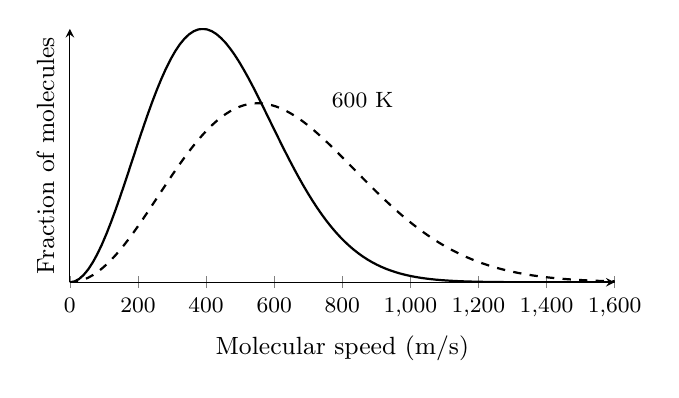
\begin{tikzpicture}
\begin{axis}[width=8.5cm,height=4.8cm,xmin=0,xmax=1600,ymin=0,axis lines=left,ytick=\empty,
  xlabel={Molecular speed (m/s)},ylabel={Fraction of molecules},samples=120,domain=0:1600,
  tick label style={font=\footnotesize},label style={font=\small}]
\addplot[thick] {x^2*exp(-x^2/(390^2))/(390^3)};
\addplot[thick,dashed] {x^2*exp(-x^2/(552^2))/(552^3)};
\node[font=\footnotesize] at (axis cs:300,0.00103) {300 K};
\node[font=\footnotesize] at (axis cs:860,0.00068) {600 K};
\end{axis}
\end{tikzpicture}

{\small\itshape Speed distributions of $\ce{N2}$ at 300 K (solid) and 600 K (dashed). Equal areas.}
\end{center}
\worked{5.1} $\ce{H2}$ and $\ce{Cl2}$ at 25 \textdegree C: same average kinetic energy; $\ce{H2}$ ($M = 2.02$) moves about $\sqrt{70.9/2.02} \approx 6$ times faster on average.

\frph ``At the same temperature the particles have the same average kinetic energy; because X has a smaller mass, its particles have a higher average speed.'' Pressure changes: ``more frequent and more forceful collisions with the walls.''

\section{Deviation from ideal gas law (Topic 3.6)}\label{t:3.6}
Real gases deviate from $PV = nRT$ when the model's assumptions fail:
\begin{itemize}
\item \emph{Attractions} (important at low temperature and for strongly attracting gases such as $\ce{NH3}$, $\ce{H2O}$): molecules are pulled back from the walls, so the measured pressure is \emph{lower} than ideal.
\item \emph{Particle volume} (important at high pressure and for large molecules): less free space than the container volume, so the measured volume (or pressure) is \emph{higher} than ideal.
\end{itemize}
Gases are most ideal at \emph{high temperature and low pressure}, and the smallest, least polarizable gases (He, $\ce{H2}$) are the most ideal.

\worked{6.1} At 1.0 atm and 300 K, which deviates more, Ne or $\ce{CH2Cl2}$ vapor? $\ce{CH2Cl2}$: it is polar and has many more electrons, so attractions between its molecules are much stronger.

\section{Solutions and mixtures (Topic 3.7)}\label{t:3.7}
A solution is a homogeneous mixture; the solute is dissolved in the solvent. Its composition is usually given as \emph{molarity}:
\[ M = \frac{\text{mol solute}}{\text{L solution}}, \qquad M_1V_1 = M_2V_2 \text{ (dilution).} \]
\begin{itemize}
\item Strong electrolytes (soluble ionic compounds, strong acids) dissociate completely. In 0.20 M $\ce{Na3PO4}$, $[\ce{Na+}] = 0.60$ M and $[\ce{PO4^3-}] = 0.20$ M.
\item To \emph{prepare} a solution: weigh the solid, dissolve it in part of the solvent in a volumetric flask, then fill to the mark. For a dilution, measure the stock with a volumetric pipet.
\end{itemize}
\worked{7.1} Mass of $\ce{CuSO4*5H2O}$ (249.7 g/mol) for 100.0 mL of 0.150 M: $0.150 \times 0.1000 = 0.0150$ mol; $\times\,249.7 = 3.75$ g.

\worked{7.2} Volume of 6.00 M $\ce{HNO3}$ needed for 500. mL of 0.300 M: $V_1 = (0.300)(500.)/6.00 = 25.0$ mL, diluted to 500. mL.

\section{Representations of solutions (Topic 3.8)}\label{t:3.8}
A good particle diagram of a solution
\begin{itemize}
\item shows the solute as separate ions (strong electrolytes) or separate molecules (nonelectrolytes such as glucose), never as intact ionic ``units'';
\item keeps the correct ratio of ions ($\ce{MgBr2}$: two $\ce{Br-}$ per $\ce{Mg^2+}$) and the correct relative concentration;
\item orients water: the O end ($\delta-$) toward cations, H atoms ($\delta+$) toward anions.
\end{itemize}
\worked{8.1} In a diagram of 0.10 M $\ce{K2SO4}$ beside 0.10 M KCl in equal volumes, the $\ce{K2SO4}$ box shows twice as many $\ce{K+}$ ions; both show the same number of anions.

\section{Separation of solutions and mixtures (Topic 3.9)}\label{t:3.9}
\begin{itemize}
\item \emph{Paper and thin-layer chromatography}: the mobile phase (solvent) moves up a stationary phase (paper or silica, both polar). Components that are attracted more to the stationary phase move less. $R_f = \dfrac{\text{distance traveled by spot}}{\text{distance traveled by solvent front}}$.
\item \emph{Column chromatography}: same principle; the component least attracted to the column comes out first.
\item \emph{Distillation}: separates liquids by volatility. The vapor, and so the first distillate, is enriched in the component with weaker IMFs.
\item \emph{Filtration} separates an undissolved solid from a liquid; it cannot separate a solution.
\end{itemize}
\worked{9.1} On polar silica with a nonpolar solvent, a spot moves 2.4 cm while the solvent front moves 8.0 cm: $R_f = 0.30$. Changing to a more polar solvent would raise $R_f$, because the solvent would now compete better for the compound.

\section{Solubility (Topic 3.10)}\label{t:3.10}
A solute dissolves well when the attractions it forms with the solvent are comparable to the solute--solute and solvent--solvent attractions that must be overcome. ``Like dissolves like'':
\begin{itemize}
\item polar and ionic solutes dissolve in polar solvents (water) through hydrogen bonding, dipole--dipole and ion--dipole attractions;
\item nonpolar solutes dissolve in nonpolar solvents (hexane, $\ce{CCl4}$) through dispersion forces;
\item in molecules with both a polar group and a nonpolar chain, solubility in water falls as the chain grows (methanol, ethanol and propanol are miscible; 1-hexanol barely dissolves).
\end{itemize}
\worked{10.1} Which dissolves better in water, $\ce{CH3COOH}$ or $\ce{C6H14}$? Acetic acid: its O--H and C=O groups hydrogen-bond with water; hexane can form only weak dispersion attractions with water, too weak to make up for breaking water's hydrogen bonds.

\section{Spectroscopy and the electromagnetic spectrum (Topic 3.11)}\label{t:3.11}
\begin{center}
\begin{tabular}{llll}\toprule
Region & Wavelength (roughly) & Molecular change & Typical use \\ \midrule
Microwave & 1 mm -- 1 m & rotation & rotational spectra \\
Infrared & 700 nm -- 1 mm & vibration (bond stretching, bending) & identifying bonds \\
Visible & 400 -- 700 nm & electronic transition & color, Beer's law \\
Ultraviolet & 10 -- 400 nm & electronic transition (can break bonds) & ozone, sunburn \\ \bottomrule
\end{tabular}
\end{center}
A colored solution absorbs the complementary color: a solution that looks green absorbs red--violet light; a blue one absorbs orange.

\section{Properties of photons (Topic 3.12)}\label{t:3.12}
\[ c = \lambda\nu \qquad E = h\nu = \frac{hc}{\lambda}, \qquad h = 6.626\times10^{-34}\unit{J\,s},\quad c = 2.998\times10^8\unit{m\,s^{-1}} \]
\begin{itemize}
\item Wavelength in meters ($1\unit{nm} = 10^{-9}\unit{m}$). Frequency in $\mathrm{s^{-1}}$ (Hz).
\item Shorter wavelength $\Leftrightarrow$ higher frequency $\Leftrightarrow$ higher energy per photon.
\item Energy per mole of photons: multiply by $N_A$.
\item A photon is absorbed only if its energy matches the gap between two energy levels; that is why each substance absorbs particular wavelengths.
\end{itemize}
\worked{12.1} Light of $\nu = 7.50\times10^{14}\unit{s^{-1}}$: $\lambda = 2.998\times10^8/7.50\times10^{14} = 4.00\times10^{-7}$ m (400 nm, violet). $E = (6.626\times10^{-34})(7.50\times10^{14}) = 4.97\times10^{-19}$ J per photon, or 299 kJ/mol.

\section{Beer--Lambert law (Topic 3.13)}\label{t:3.13}
\[ A = \varepsilon b c \]
$A$ is absorbance (no units), $\varepsilon$ the molar absorptivity ($\mathrm{M^{-1}\,cm^{-1}}$, a property of the solute at one wavelength), $b$ the path length (cm), $c$ the concentration (M).
\begin{itemize}
\item A \emph{calibration curve} of $A$ against $c$ for standards is a straight line through the origin with slope $\varepsilon b$. Read an unknown's concentration from its absorbance.
\item Measure at $\lambda_{\max}$, where $\varepsilon$ is largest, for the greatest sensitivity.
\item \emph{Blank} the instrument with the solvent so that only the solute's absorbance is measured.
\end{itemize}
\textbf{Error analysis.} Anything that removes light other than absorption by the solute (fingerprints, scratches, bubbles, a colored impurity) raises $A$ and makes the calculated $c$ too high. Diluting the sample (water in the cuvette) lowers $A$ and makes $c$ too low.

\worked{13.1} A standard of $4.0\times10^{-5}$ M gives $A = 0.320$ in a 1.00 cm cell, so $\varepsilon = 8.0\times10^3\unit{M^{-1}\,cm^{-1}}$. An unknown with $A = 0.200$ has $c = 0.200/8.0\times10^3 = 2.5\times10^{-5}$ M.

\section{Lab skills and free-response technique}\label{t:lab}
\begin{itemize}
\item \emph{Molar volume / gas collection labs}: subtract water's vapor pressure; convert mL to L and \textdegree C to K; level the water inside and outside the collection tube so the gas is at atmospheric pressure.
\item \emph{Solution preparation}: volumetric flask for the final volume; analytical balance for the solute; pipet for aliquots. A graduated cylinder is less precise.
\item \emph{Spectrophotometry}: blank, choose $\lambda_{\max}$, make standards that bracket the unknown, plot $A$ vs.\ $c$.
\item \emph{Chromatography}: mark the origin in pencil, keep the spots above the solvent level, and measure to the center of each spot.
\end{itemize}
Free-response questions in this unit almost always ask you to (1) identify the IMF, (2) compare strengths with a particle-level reason, and (3) connect to a property. In gas problems, show $PV = nRT$ with units substituted.

\clearpage
\section*{Summary: Unit 3 on one page}
Use this page the night before. For any row you cannot explain from memory, reread its section and redo its worked example.

\begin{longtable}{@{}p{0.11\linewidth}p{0.40\linewidth}p{0.43\linewidth}@{}}\toprule
\S{} / Topic & Must know & Key equations and tests \\ \midrule
1 / 3.1 & Dispersion, dipole--dipole, H-bond, ion--dipole & size first, then type, then shape \\[3pt]
2 / 3.2 & Four solid types and their properties & conductivity, melting point, hardness \\[3pt]
3 / 3.3 & Phase particle models; vapor pressure & same $T$ = same KE \\[3pt]
4 / 3.4 & $PV = nRT$; Dalton; molar mass from density & $M = dRT/P$; $P_i = X_iP$ \\[3pt]
5 / 3.5 & KMT postulates; Maxwell--Boltzmann & lighter $\Rightarrow$ faster at same $T$ \\[3pt]
6 / 3.6 & Attractions lower $P$; volume raises $V$ & ideal at high $T$, low $P$ \\[3pt]
7 / 3.7 & Molarity; dilution; ion concentrations & $M = n/V$; $M_1V_1 = M_2V_2$ \\[3pt]
8 / 3.8 & Ions separate; ratios; water orientation & O toward cations, H toward anions \\[3pt]
9 / 3.9 & Chromatography; distillation & $R_f$; weaker IMF elutes / distills first \\[3pt]
10 / 3.10 & Like dissolves like & chain length lowers water solubility \\[3pt]
11 / 3.11 & MW rotation, IR vibration, UV--vis electronic & complementary colors \\[3pt]
12 / 3.12 & Photon energy & $c = \lambda\nu$, $E = h\nu = hc/\lambda$ \\[3pt]
13 / 3.13 & Calibration line; $\lambda_{\max}$; error direction & $A = \varepsilon bc$ \\ \bottomrule
\end{longtable}

\textbf{Constants.} $R = 0.08206\unit{L\,atm\,mol^{-1}\,K^{-1}} = 8.314\unit{J\,mol^{-1}\,K^{-1}}$; $1\unit{atm} = 760\unit{torr} = 101.3\unit{kPa}$; $h = 6.626\times10^{-34}\unit{J\,s}$; $c = 2.998\times10^8\unit{m\,s^{-1}}$; $N_A = 6.022\times10^{23}\unit{mol^{-1}}$.
\end{document}
